\documentclass[border=2pt, 12pt]{standalone}

\usepackage{tikz}
    \usetikzlibrary{math, calc, arrows.meta}
\usepackage{siunitx}

\begin{document}
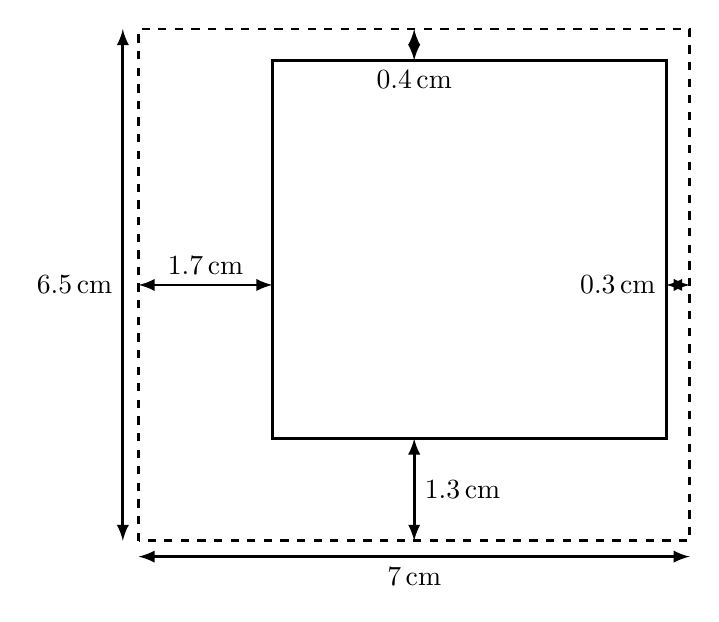
\begin{tikzpicture}[line width=1pt]
    \tikzmath{
        \figweight=7;
        \figheight=6.5;
        \axleft=1.7;
        \axright=0.3;
        \axbottom=1.3;
        \axtop=0.4;
    }

    \coordinate (O) at (0, 0);
    \draw [dashed] (O) rectangle ++(\figweight, \figheight);
    \draw ($ (O) + (\axleft, \axbottom) $) rectangle ($ (O) + ({\figweight-\axright}, {\figheight-\axtop}) $);

    % figure
    \draw [latex-latex] ($ (O) + (-0.2, 0) $) -- ++(0, \figheight)
    node [left, midway] {$ \qty{\figheight}{\centi\meter} $};
    \draw [latex-latex] ($ (O) + (0, -0.2) $) -- ++(\figweight, 0)
    node [below, midway] {$ \qty{\figweight}{\centi\meter} $};

    % axes
    \draw [latex-latex] (0, \figheight/2) -- (\axleft, \figheight/2)
    node [above, midway] {$ \qty{\axleft}{\centi\meter} $};
    \draw [latex-latex] (\figweight/2, 0) -- (\figweight/2, \axbottom)
    node [right, midway] {$ \qty{\axbottom}{\centi\meter} $};
    \draw [latex-latex] (\figweight/2, \figheight) -- (\figweight/2, \figheight-\axtop)
    node [below] {$ \qty{\axtop}{\centi\meter} $};
    \draw [latex-latex] (\figweight, \figheight/2) -- (\figweight-\axright, \figheight/2)
    node [left] {$ \qty{\axright}{\centi\meter} $};
\end{tikzpicture}
\end{document}